\documentclass[10pt,border=5pt]{standalone}
\usepackage[T1]{fontenc}
\usepackage{lmodern,amsmath,amssymb,mathrsfs,tikz}
\usetikzlibrary{arrows.meta,positioning,calc}
\definecolor{ink}{HTML}{192536}
\definecolor{blue}{HTML}{2E70AE}
\definecolor{gold}{HTML}{A66A15}
\definecolor{green}{HTML}{28764D}
\definecolor{red}{HTML}{B43D3D}
\newcommand{\C}{\mathbb C}
\newcommand{\R}{\mathcal R}
\newcommand{\Lr}{\mathcal L_{\mathrm{res}}}
\newcommand{\Prs}{\mathcal P_{\mathrm{res}}}
\newcommand{\Tr}{T_{\mathrm{resp}}}
\newcommand{\rr}{\rho_{\mathrm{res}}}
\tikzset{every node/.style={font=\small,text=ink,align=center},
 box/.style={draw=blue,fill=blue!4,rounded corners=3pt,line width=.7pt,inner sep=7pt},
 goldbox/.style={box,draw=gold,fill=gold!5},
 greenbox/.style={box,draw=green,fill=green!5},
 redbox/.style={box,draw=red,fill=red!4},
 edge/.style={-{Stealth[length=4pt]},draw=ink,line width=.7pt},
 heading/.style={font=\small\bfseries},
 note/.style={font=\small,text=ink!85}}

\begin{document}
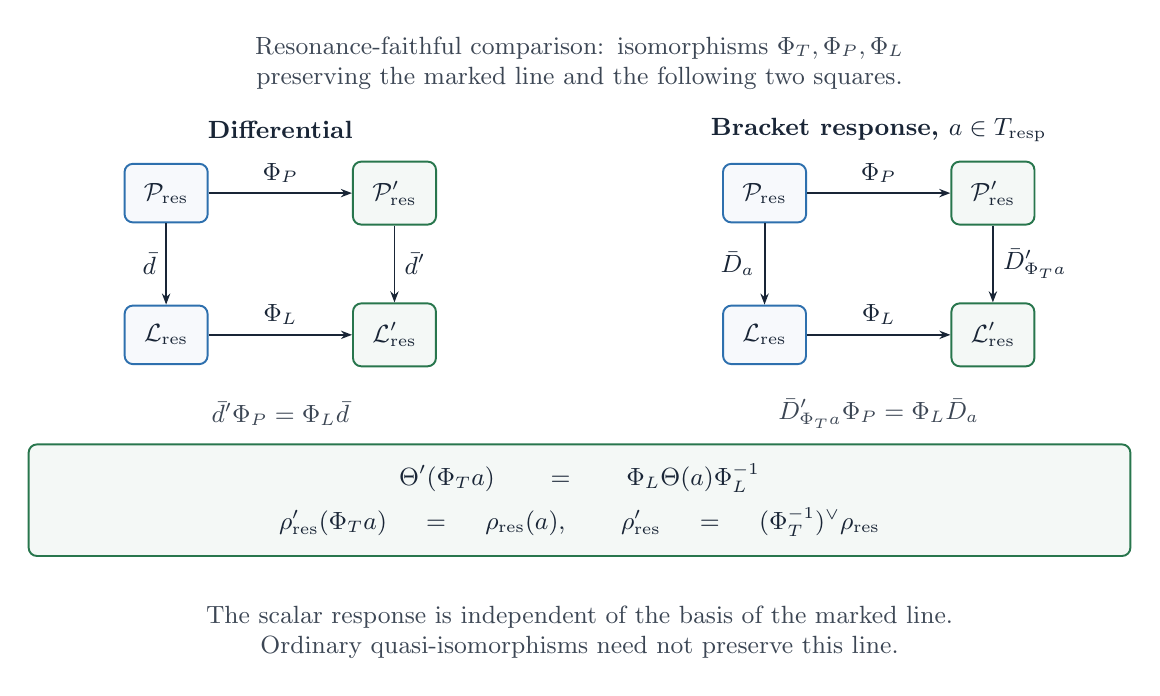
\begin{tikzpicture}
\node[note,text width=13.5cm] at (3.8,1.45)
 {Resonance-faithful comparison: isomorphisms $\Phi_T,\Phi_P,\Phi_L$\\
 preserving the marked line and the following two squares.};
\node[heading] at (0,0.6) {Differential};
\node[heading] at (7.6,0.6) {Bracket response, $a\in\Tr$};
\node[box] (p) at (-1.45,-.2) {$\Prs$};
\node[greenbox] (pp) at (1.45,-.2) {$\mathcal P'_{\mathrm{res}}$};
\node[box] (l) at (-1.45,-2) {$\Lr$};
\node[greenbox] (lp) at (1.45,-2) {$\mathcal L'_{\mathrm{res}}$};
\draw[edge] (p)--node[above]{$\Phi_P$}(pp);
\draw[edge] (l)--node[above]{$\Phi_L$}(lp);
\draw[edge] (p)--node[left]{$\bar d$}(l);
\draw[edge] (pp)--node[right]{$\bar d'$}(lp);
\node[box] (q) at (6.15,-.2) {$\Prs$};
\node[greenbox] (qp) at (9.05,-.2) {$\mathcal P'_{\mathrm{res}}$};
\node[box] (m) at (6.15,-2) {$\Lr$};
\node[greenbox] (mp) at (9.05,-2) {$\mathcal L'_{\mathrm{res}}$};
\draw[edge] (q)--node[above]{$\Phi_P$}(qp);
\draw[edge] (m)--node[above]{$\Phi_L$}(mp);
\draw[edge] (q)--node[left]{$\bar D_a$}(m);
\draw[edge] (qp)--node[right]{$\bar D'_{\Phi_Ta}$}(mp);
\node[note] at (0,-3) {$\bar d'\Phi_P=\Phi_L\bar d$};
\node[note] at (7.6,-3) {$\bar D'_{\Phi_Ta}\Phi_P=\Phi_L\bar D_a$};
\node[greenbox,text width=13.5cm] (theta) at (3.8,-4.1)
 {$\Theta'(\Phi_Ta)=\Phi_L\Theta(a)\Phi_L^{-1}$\\[5pt]
 $\rho'_{\mathrm{res}}(\Phi_Ta)=\rr(a),\qquad
 \rho'_{\mathrm{res}}=(\Phi_T^{-1})^\vee\rr$};
\node[note,text width=13.5cm,below=5mm of theta]
 {The scalar response is independent of the basis of the marked line.\\
 Ordinary quasi-isomorphisms need not preserve this line.};
\end{tikzpicture}
\end{document}
